\begin{frame}
    \frametitle{\problemtitle}
    \begin{block}{Problem}
        Given $n$ axis-aligned rectangles, determine whether there is a line
        intersecting or touching all of them.
    \end{block}
	\begin{overprint}
		\onslide<1|handout:0>
		\centering
		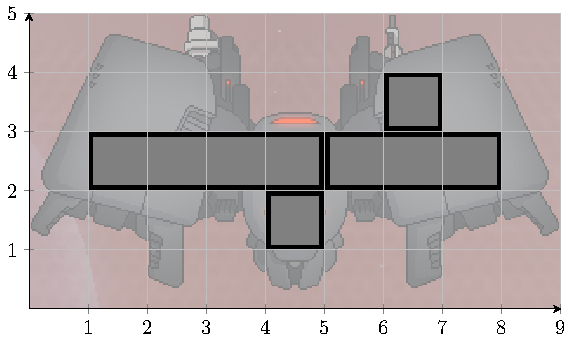
\includegraphics[height=0.4\textheight]{example1}
		\onslide<2|handout:0>
		\centering
		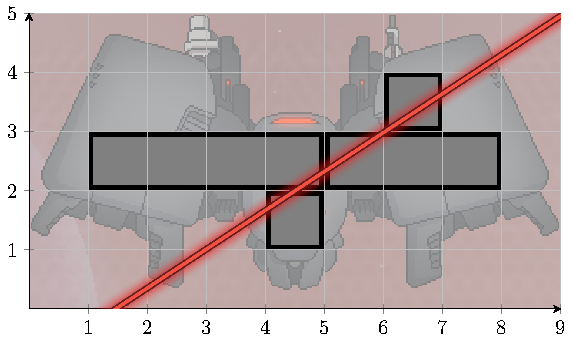
\includegraphics[height=0.4\textheight]{example2}
		\onslide<3|handout:0>
		\centering
		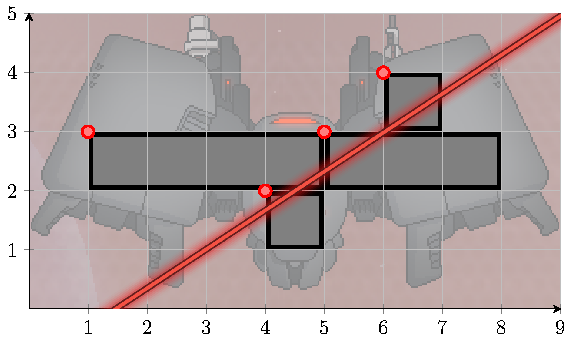
\includegraphics[height=0.4\textheight]{example3}
		\onslide<4-5|handout:0>
		\centering
		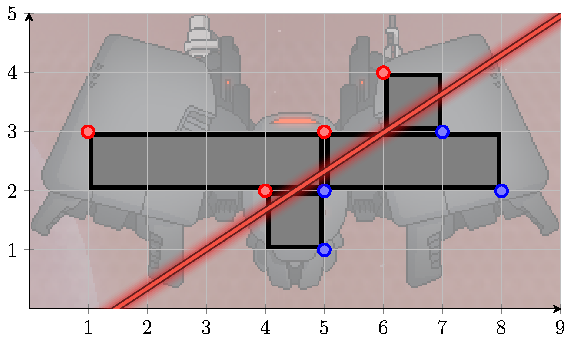
\includegraphics[height=0.4\textheight]{example4}
	\end{overprint}
    \pause
    \begin{block}{Observation}
    	\begin{itemize}
    	\item<+-> If the solution line has positive slope, then:
    	 	\begin{itemize}
    		\item<+-> it passes below the top left corners of every rectangle,
    		\item<+-> it passes over the bottom right corner of every rectangle.
    		\end{itemize}
    	\item<+-> For lines with negative slope, something similar holds.
    	\end{itemize}
    \end{block}
\end{frame}

\begin{frame}
    \frametitle{\problemtitle}
    \begin{block}{Problem}
        Given $n$ axis-aligned rectangles, determine whether there is a line
        intersecting or touching all of them.
    \end{block}
    \centering
    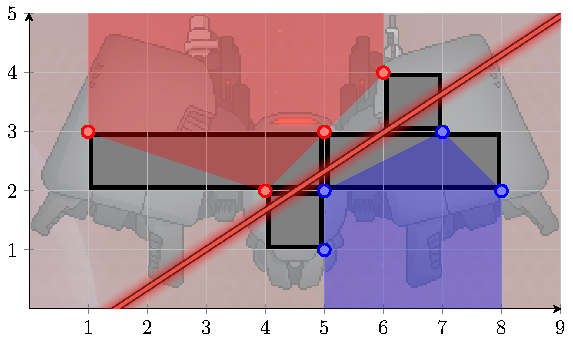
\includegraphics[height=0.4\textheight]{example5}
    \begin{block}{Observation}
    	Use the upper convex hull of the red points and lower convex
            hull of the blue points.
        \pause
        \begin{itemize}
        \item<+-> A line that passes in between intersects all rectangles.
        \item<+-> A line inside a convex hull goes above/below a red/blue point.
        \end{itemize}
    \end{block}
\end{frame}

\begin{frame}
    \frametitle{\problemtitle}
	\begin{block}{Problem}
        Given $n$ axis-aligned rectangles, determine whether there is a line
        intersecting or touching all of them.
    \end{block}

    \begin{block}{Solution}
        \begin{itemize}
            \item<+-> First check for lines with positive slope:
            	\begin{itemize}
            	\item Compute the lower convex hull of all top left corners.
            	\item Compute the upper convex hull of all bottom right corners.
            	\item Check (in linear time) whether these intersect.
            	\end{itemize}
            \item<+-> In a similar way, check for lines with negative slope.
            \item<+-> Also check for vertical lines.
            \item<+-> Total running time: $\mathcal{O}(n \log n)$.
        \end{itemize}
    \end{block}
    \solvestats
\end{frame}
